\chapter{Musicality of the solutions}\label{chapter:musicality}
This last chapter deals with the musicality of the solutions. While the aim of the previous chapter was to find out how best to adjust the preferences to reflect Fux's will, the aim of this chapter is to see what FuxCP is capable of (using a given preference management technique). We first have a look at basic solutions, i.e. compositions where species are not mixed, as in most of Fux's examples, then we will have a look at what happens when we try to leave Fux's writing style by using preferences, and finally we discuss a bit about cross-species compositions.

\section{Looking at the results of single species compositions}
Composing with three voices, one of which is the \cf, one of which is a counterpoint of the first species, and the last of which is a counterpoint of any species, is the basic situation of writing counterpoint, as Fux explains in his teaching of counterpoint. In this first sub-section, therefore, we shall consider five basic counterpoints to a \cfs in C.

\begin{figure}[h!]
    \centering
    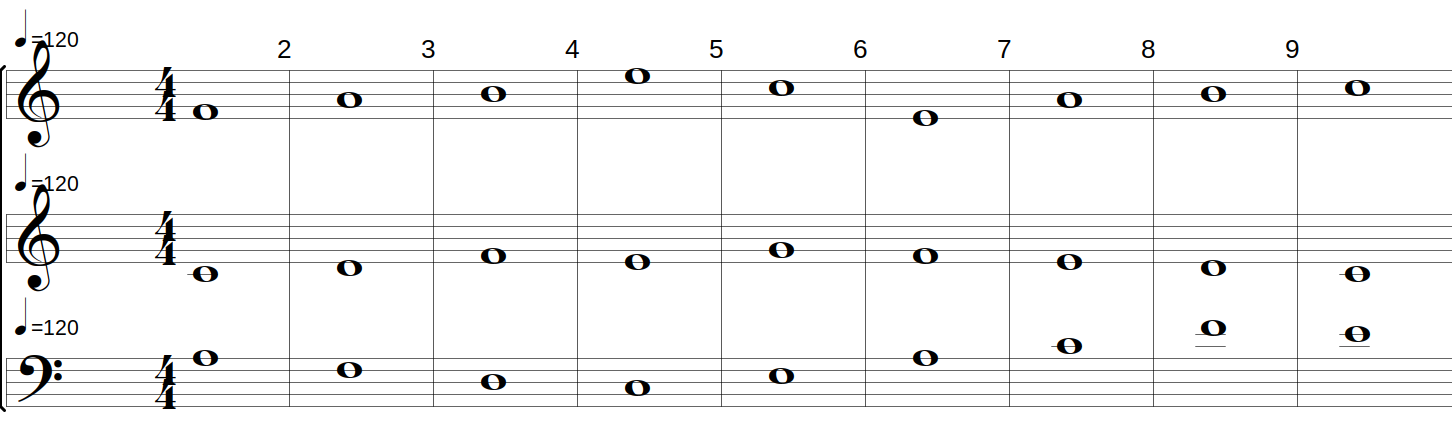
\includegraphics[width=1\textwidth]{Images/Musicality/simple-test-1sp.png}
    \caption{Simple first species composition with three voices. Click \href{https://youtu.be/qIresNFcmWY}{here} to listen.}
    \label{fig:simple-test-1sp}
\end{figure}
\begin{figure}[h!]
    \centering
    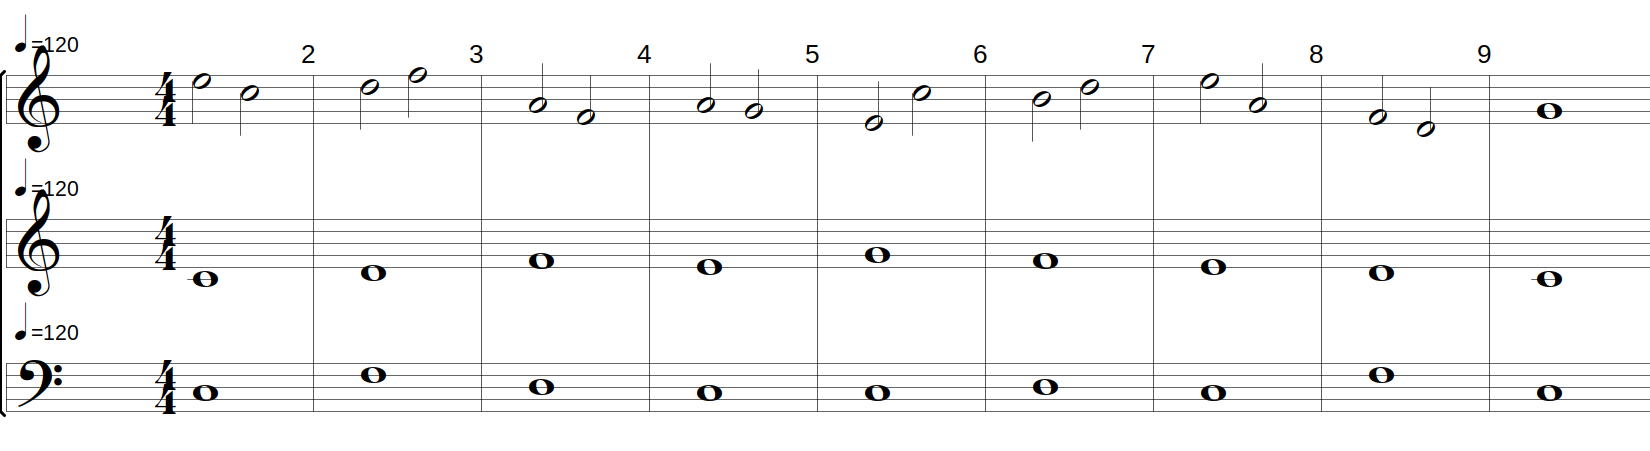
\includegraphics[width=1\textwidth]{Images/Musicality/simple-test-2sp.png}
    \caption{Simple second species composition with three voices. Click \href{https://example.com/}{here} to listen.}
    \label{fig:simple-test-2sp}
\end{figure}
\begin{figure}[h!]
    \centering
    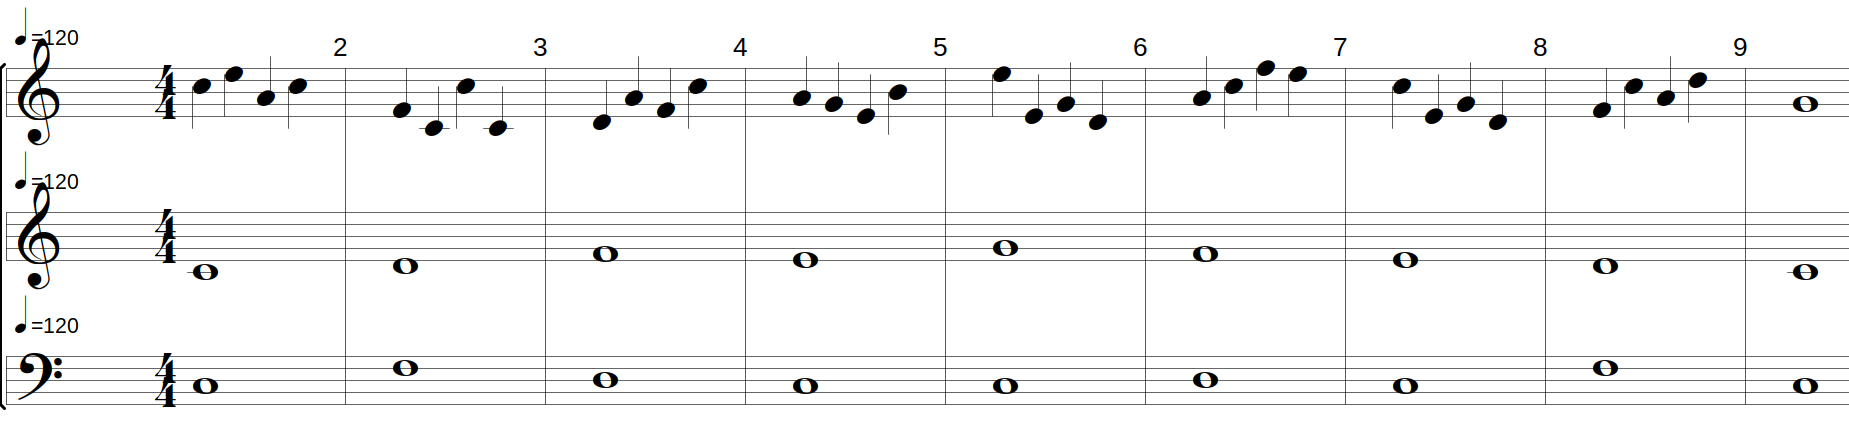
\includegraphics[width=1\textwidth]{Images/Musicality/simple-test-3sp.png}
    \caption{Simple third species composition with three voices. Click \href{https://youtu.be/r6MaQHyTLs8}{here} to listen.}
    \label{fig:simple-test-3sp}
\end{figure}
\begin{figure}[h!]
    \centering
    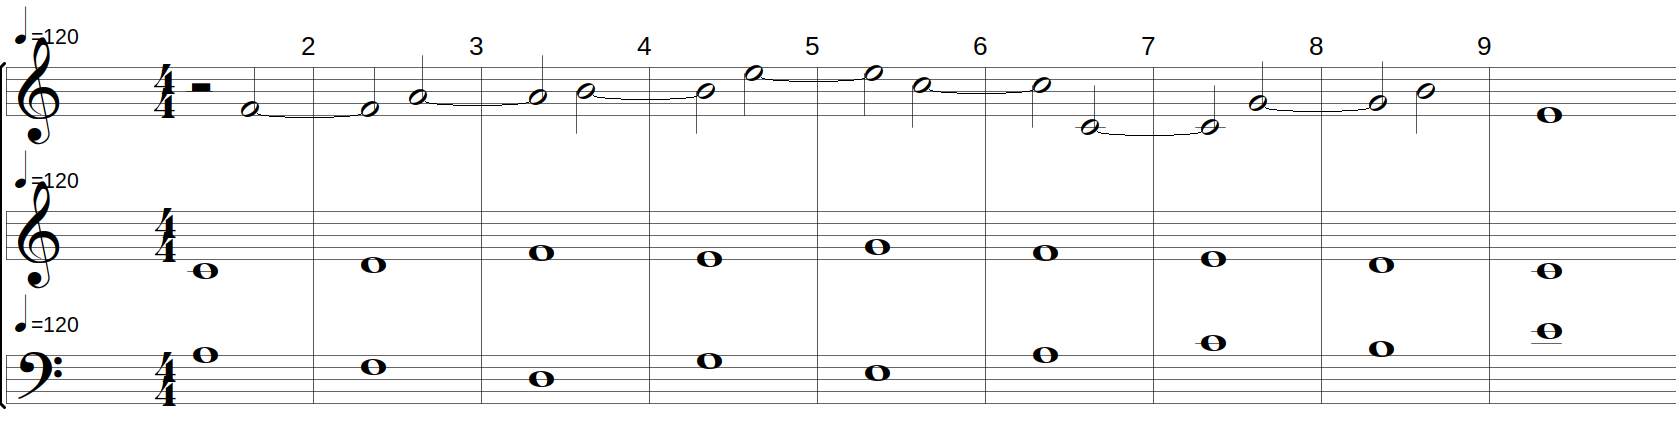
\includegraphics[width=1\textwidth]{Images/Musicality/simple-test-4sp.png}
    \caption{Simple fourth species composition with three voices. Click \href{https://youtu.be/gcGoXKLcV_I}{here} to listen.}
    \label{fig:simple-test-4sp}
\end{figure}
\begin{figure}[h!]
    \centering
    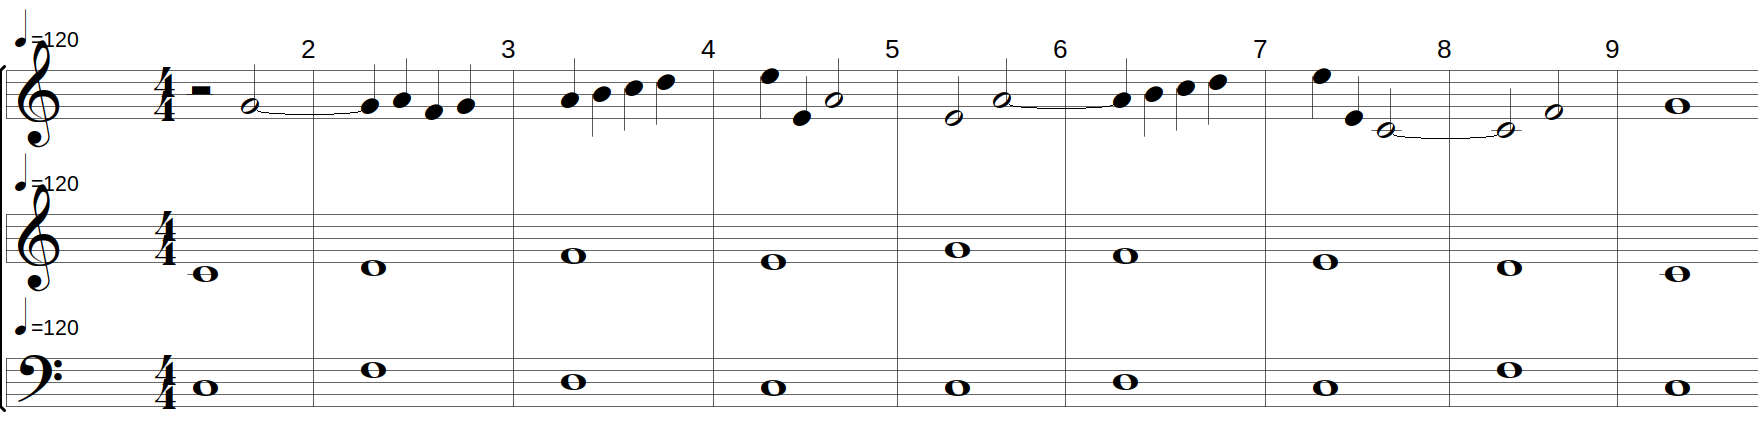
\includegraphics[width=1\textwidth]{Images/Musicality/simple-test-5sp.png}
    \caption{Simple fifth species composition with three voices. Click \href{https://youtu.be/BSAKEjvFdoo}{here} to listen.}
    \label{fig:simple-test-5sp}
\end{figure}

Looking at all these examples, we can draw the following conclusions: 

\begin{itemize}
    \item Fux was right when he said that three-part composition is much richer than two-part composition (without even having to mix the species). The addition of the third voice adds depth, dimension and colour, and the problems of monotony that arise in the automation of two-part writing seem to have been partially solved. With two voices, if one voice repeated itself, the composition as a whole suffered from repetitiveness. With three voices, if one voice repeats itself, because the other voices change, this creates variation. In fact, we could say more, as this is in keeping with the general idea of counterpoint, which is that patterns repeat and alternate. In this case, of course, the repetitions are due to chance (remember that all the rules, except the preference for variety, apply to a maximum of one measure, so the solver does not have an overall view of the composition), but in the future we could add rules to encourage these repetitions and variations, or even to encourage the voices to respond to each other! 
    \item Too often the final chord is not conclusive. This could be solved by an additional rule to be defined. It is surprising that Fux does not cover this case in his rules. In fact, the only rules he mentions for the final chord are "no minor third" and "no tenth". Apparently that's not enough.
    \item It would be difficult to call these compositions masterpieces. However, they stand up well enough to be used as a basis, and with a few personal improvements on the part of the composer, they can be expanded and improved as much as desired. For example, by changing the few notes that don't go together so well, by modifying the harmonies or by adding different rhythms. The result of the basic counterpoint is therefore more than satisfactory and can be considered a success.
\end{itemize}


\section{Trying custom costs}
Below is an example of the difference between a counterpoint of the first species, using Fux's preferences (more precisely, using a lexicographic search with default preferences as defined in Section \ref{section:lexicographic-order}), and a counterpoint in which personal preferences were expressed. These preferences were: to use as few contrary motions as possible, and as many oblique and direct motions as possible. Prioritising this preference (placing it first in the lexicographic order), then prioritising melodic intervals (maintaining a preference for small melodic intervals, as in \gap), then prioritising variety, and then placing all the other preferences at the penultimate level of the lexicographic order, with the exception of the preference for no successive perfect consonance, which was placed at the very last level.

The search has not been stopped manually; we leave it running until it finds the best solution according to the defined preferences.

The aim of this experiment is twofold: to show that the preferences can have a big impact on the resulting solution, giving the composer a lot of room for manoeuvre in their composition (this was already partially demonstrated in the previous chapter), and to obtain a solution that differs from Fux's compositions. In particular, these small changes in preferences were made to obtain a more monotonous solution, with fewer twists than the Fux-like solutions (for example, for transitions between two parts of a composition, for more quiet moments, ...).

The results of this experiment can be found in figures \ref{fig:musicality-1sp-fux} and \ref{fig:musicality-1sp-custom}.
\begin{figure}[h!]
    \centering
    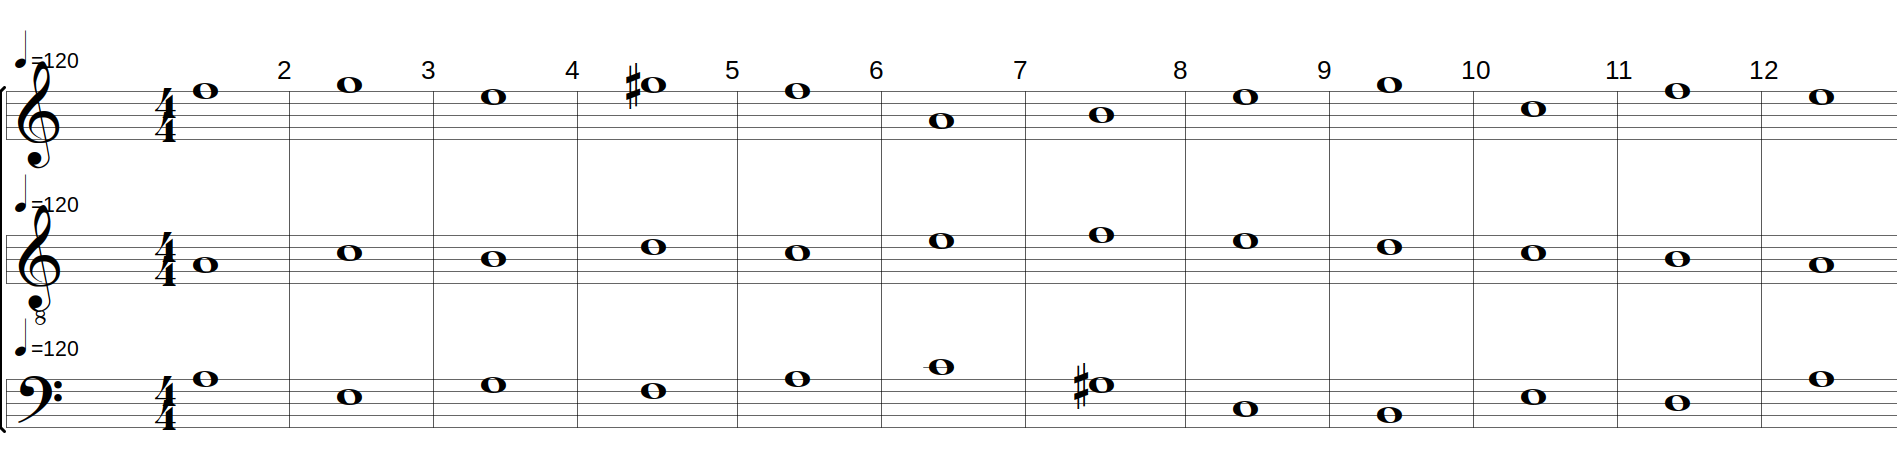
\includegraphics[width=1\textwidth]{Images/Musicality/musicality-1sp-fux-pref.png}
    \caption{Example of a first species counterpoint in three-part composition with Fux's preferences. Click \href{https://youtu.be/rXGOzidniA0}{here} to listen.}
    \label{fig:musicality-1sp-fux}
\end{figure}

\begin{figure}[h!]
    \centering
    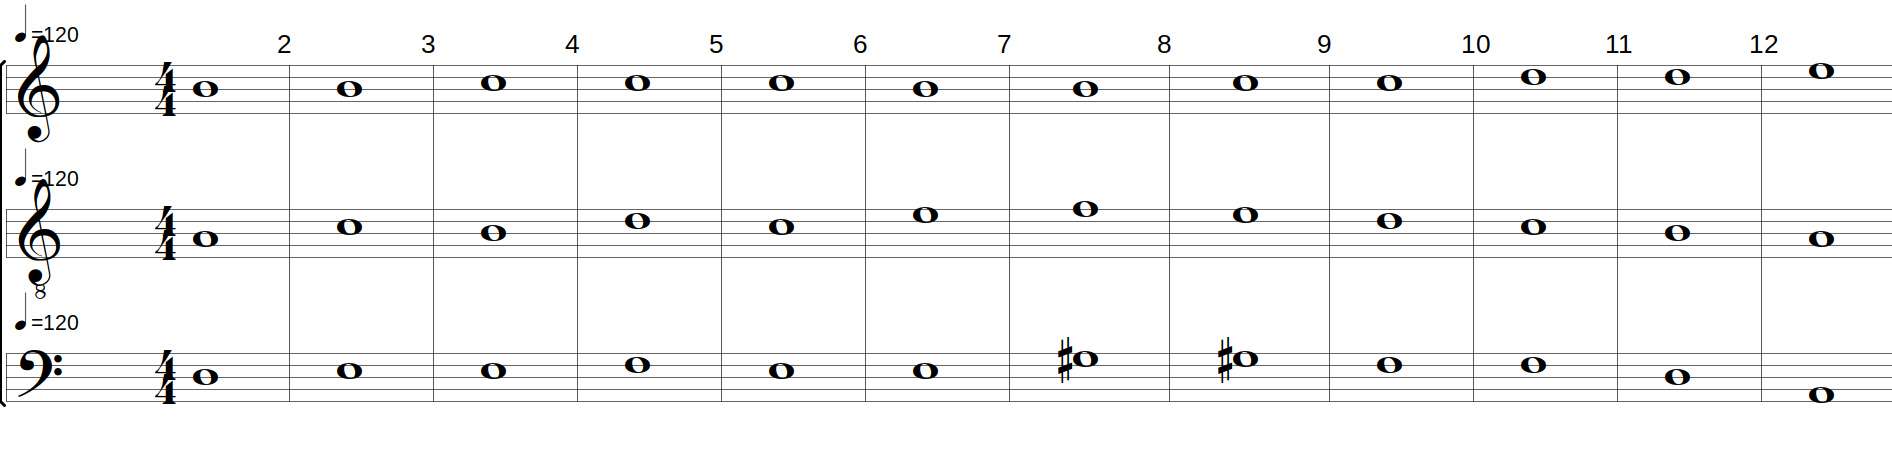
\includegraphics[width=1\textwidth]{Images/Musicality/musicality-1sp-custom-pref.png}
    \caption{Example of a first species counterpoint in three-part composition with custom preferences. Click \href{https://youtu.be/aWmkHdcuook}{here} to listen.}
    \label{fig:musicality-1sp-custom}
\end{figure}

The result is striking, as the Fux-like solution simply sounds like... Fux, and the custom solution is completely in line with its aim, which was to create a composition that is more monotonous and where there is less sense of things happening. This example shows something interesting: with the same set of hard constraints (the mandatory rules of Fux), it is possible, thanks to preferences, to make a variety of personal choices that still sound good but deviate from the traditional style of Fux. 

\section{Analysing the results of mixing species}
If there's one thing that's clear about multi-species composition, it's that it's a truly unpredictable art. It has already been discussed in the \ref{section:time-to-find-a-solution} section that the different interactions between species, voice ranges and \textit{cantus firmi} can take more or less time in terms of solver efficiency. This is also true for the quality of the solutions, and there are times when the solver gives completely correct results, and times when the solution leaves a lot to be desired. This lack of musical quality in the solutions was not the case when we were composing single species counterpoints (without mixing the species), and is something that emerges when combining species. The most plausible hypothesis is that the solver is unable to produce a solution that is \textit{always} beautiful when combining species precisely because Fux has never given any rules specifying how to combine species. We can only hope that such rules exist in the 3rd chapter of his book, or else we'll have to either extrapolate from existing rules or take inspiration from other authors to create these rules.

Below (Figures \ref{fig:musicality-5sp-la} and \ref{fig:musicality-5sp-do}) are two examples of counterpoint generated by FuxCP. Both combine counterpoint of the second kind and counterpoint of the fifth species. The search ran for three minutes before being interrupted.

\begin{figure}[h!]
    \centering
    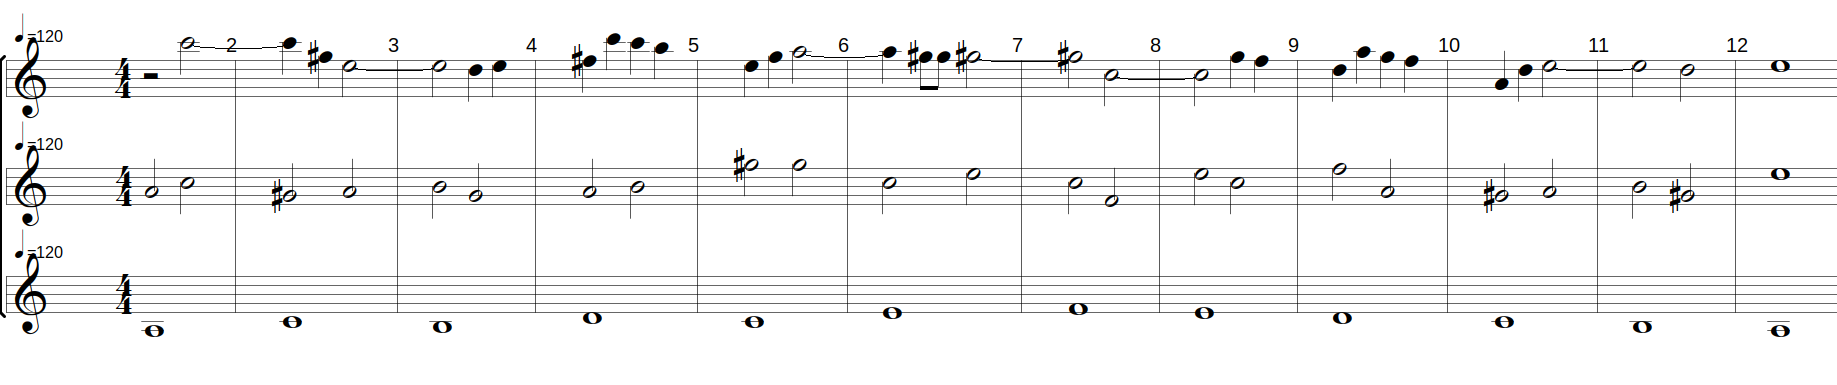
\includegraphics[width=1\textwidth]{Images/Musicality/musicality-5sp-la.png}
    \caption{Example of a generated counterpoint using a second species counterpoint and a fifth species counterpoint, with in an A scale.}
    \label{fig:musicality-5sp-la}
\end{figure}

\begin{figure}[h!]
    \centering
    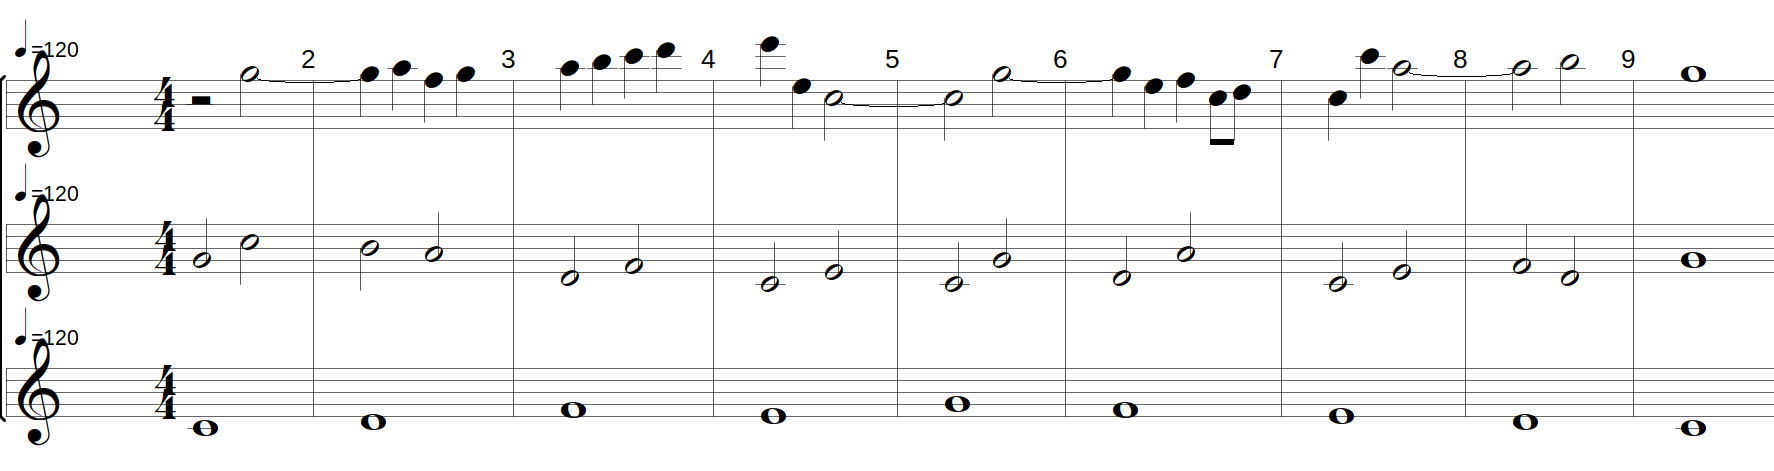
\includegraphics[width=1\textwidth]{Images/Musicality/musicality-5sp-do.png}
    \caption{Example of a generated counterpoint using a second species counterpoint and a fifth species counterpoint, with in a C scale.}
    \label{fig:musicality-5sp-do}
\end{figure}